%% beamerthemeImperialPoster v1.0 2016/10/01
%% Beamer poster theme created for Imperial College by LianTze Lim (Overleaf)
%% LICENSE: LPPL 1.3
%%
%% This is the example poster demonstrating use
%% of the Imperial College Beamer Poster Theme
\documentclass[xcolor={table}]{beamer}
%% Possible paper sizes: a0, a0b, a1, a2, a3, a4 (although Imperial College posters are usually A0 or A1).
%% Possible orientations: portrait, landscape
%% Font sizes can be changed using the scale option.
\usepackage[size=a0,orientation=portrait,scale=1.55]{beamerposter}
\usepackage{src/beamercolorthemeImperialWhite}
%\usepackage{src/beamercolorthemeImperialBlack}
%\usepackage{src/beamercolorthemeImperialDarkBlue}
%\usepackage{src/beamercolorthemeImperialLightBlue}
\usepackage{src/beamerthemeImperialPoster}
\usepackage{graphicx}
\graphicspath{{images/}}

\usepackage{siunitx}

\title{Signal Optimization for Wireless Information and Power Transmission}

\author{\textit{Author:} Yang Zhao (yang.zhao18@imperial.ac.uk) \\
        \textit{Supervisor:} Dr Bruno Clerckx and Dr Morteza Varasteh}

\addbibresource{sample.bib}


\begin{document}
\begin{frame}[fragile=singleslide,t]\centering

\maketitle

\begin{columns}[onlytextwidth,T]

%%%% First Column
\begin{column}{.47\textwidth}

\begin{block}{Motivation}
Energy-constrained wireless devices are conventionally powered by batteries. However, the development of large-scale networks as Internet-of-Things (IoT) is strictly restricted by its limited working time and frequent recharging or replacement. Although Wireless Power Transfer (WPT) via inductive coupling has enjoyed some success in real-world applications, it is impractical for most devices on the move since the operation range is very short. As a promising alternative, the Radio-Frequency (RF) wave is typically with lower power level (\si{\uW} to \si{W}) but larger coverage (up to hundreds of \si{m}) \citep{Ng2019}. Interestingly, it indeed carries both information and energy simultaneously, with the potential to power billions of mobile nodes wirelessly while keeping them connected. The recent revolution in harvester model and the significant power drop of electronics bring more possibility to the research on Wireless Information and Power Transfer (WIPT) via RF signals.
\end{block}

%\begin{block}{Architecture}
%From the perspective of WPT, the end-to-end power transfer efficiency writes as:
%
%\begin{equation}\label{eqn:power_utilization_efficiency}
%  e = \frac{{{P_{{\text{dc}},{\text{ST}}}}}}{{P_{{\text{dc}}}^t}} = \underbrace {\frac{{P_{{\text{rf}}}^t}}{{P_{{\text{dc}}}^t}}}_{{e_1}} \cdot \underbrace {\frac{{P_{{\text{rf}}}^r}}{{P_{{\text{rf}}}^t}}}_{{e_2}} \cdot \underbrace {\frac{{P_{{\text{dc}}}^r}}{{P_{{\text{rf}}}^r}}}_{{e_3}} \cdot \underbrace {\frac{{{P_{{\text{dc}},{\text{ST}}}}}}{{P_{{\text{dc}}}^r}}}_{{e_4}}
%\end{equation}
%
%\begin{figure}
%  \centering
%    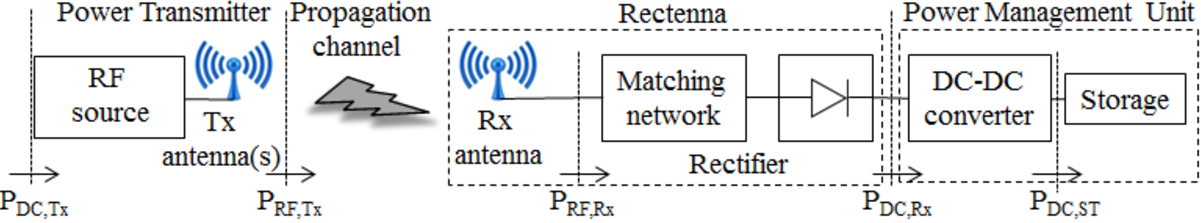
\includegraphics[width=\textwidth]{wpt_block_diagram}
%  \caption{\textit{Block diagram of a conventional far-field WPT architecture \citep{Clerckx2018a}. We particularly focus on the rectenna behavior.}}
%  \label{fig:wpt-block-diagram}
%\end{figure}
%
%The RF-to-DC conversion efficiency ${e_3}$ is related to \textbf{rectenna model} and \textbf{waveform design}.
%\end{block}

\begin{block}{Rectenna Model}
A rectenna receives electromagnetic power with antenna and convert it to electric power with rectifier.
\begin{figure}
  \centering
    \includegraphics[width=0.8\textwidth]{rectenna_behavior}
  \caption{A single diode rectifier (left) and diode $I -- V$ characteristics \cite{Clerckx2019}}
  \label{fig:rectenna_circuit}
\end{figure}
\begin{itemize}
  \item Diodes account for nonlinearity
  \item Approximate diode characteristic equation by Taylor series
  \item Truncate the result to ${n_o}$-th order
  \begin{itemize}
    \item \textbf{diode linear model (${n_o} = 2$)} is the conventional perspective that assumes the total output power is the sum of the subband power. It omits the rectifier nonlinearity and is typically suitable for a very low input power (below -30 dBm).
    \item \textbf{diode nonlinear model (${n_o} > 2$)} considers the contributions of higher order terms to the harvested power. It captures the diode nonlinear behavior with the product terms that consist of contributions from different frequencies. The model is accurate for the power regime between -30 and 0 dBm.
  \end{itemize}
\end{itemize}
\end{block}

\begin{sidefigure}
\includegraphics[width=\hsize]{example-image-golden-upright}
\caption{Lorem ipsum dolor sit amet, consectetuer adipiscing elit. In nunc nisl, pharetra et, lacinia non, pellentesque sit amet, tellus. Sed tempus. In egestas. Maecenas aliquam libero vitae leo. Donec consectetuer. Pellentesque ultrices feugiat enim. Morbi tempus tortor non metus. Quisque vitae metus. Nulla justo. Pellentesque laoreet dui a felis bibendum blandit. Quisque commodo. Cras luctus vestibulum leo. Quisque varius mauris vel diam. Aenean quis erat. Vestibulum mauris. Suspendisse potenti. Vivamus consectetuer massa et nunc. Aliquam ornare risus eu risus. Suspendisse molestie urna vitae augue.

Aliquam erat volutpat. Duis at sapien vestibulum mi sollicitudin rutrum.}
\end{sidefigure}

\begin{block}{Header}
Lorem ipsum dolor sit amet, consectetuer adipiscing elit. In nunc nisl, pharetra et, lacinia non, pellentesque sit amet, tellus. Sed tempus. In egestas. Maecenas aliquam libero vitae leo. Donec consectetuer. Pellentesque ultrices feugiat enim. Morbi tempus tortor non metus. Quisque vitae metus. Nulla justo. Pellentesque laoreet dui a felis bibendum blandit. Quisque commodo. Cras luctus vestibulum leo. Quisque varius mauris vel diam.  Aenean quis erat. Vestibulum mauris. Suspendisse potenti. Vivamus consectetuer massa et nunc.
\end{block}

\begin{table}
\begin{tabularx}{\linewidth}{  X  X  }
\toprule
\textbf{Table header (bold)} & \textbf{Table header (bold)} \\
\midrule
Table header (normal) & Table header (normal) \\
\midrule
Table header (normal) & Table header (normal) \\
\midrule
Table header (normal) & Table header (normal) \\
\bottomrule
\end{tabularx}
\end{table}

\begin{block}{Acknowledgements}
Lorem ipsum dolor sit amet, consectetuer adipiscing elit. In nunc nisl, pharetra et, lacinia non, pellentesque sit amet, tellus. Sed tempus. In egestas. Maecenas aliquam libero vitae leo. Donec consectetuer. Pellentesque ultrices feugiat enim. Morbi tempus tortor non metus. Quisque vitae metus. Nulla justo.
\end{block}

\end{column}


%%%% Second Column
\begin{column}{.47\textwidth}

\begin{block}{Header}
Lorem ipsum dolor sit amet, consectetuer adipiscing elit. In nunc nisl, pharetra et, lacinia non, pellentesque sit amet, tellus. Sed tempus. In egestas. Maecenas aliquam libero vitae leo. Donec consectetuer. Pellentesque ultrices feugiat enim. Morbi tempus tortor non metus. Quisque vitae metus. Nulla justo. Pellentesque laoreet dui a felis bibendum blandit. Quisque commodo.
Cras luctus vestibulum leo. Quisque varius mauris vel diam. Aenean quis erat. Vestibulum mauris. Suspendisse potenti. Vivamus consectetuer massa et nunc.
\end{block}

\begin{block}{Header}
\begin{itemize}
\item Lorem ipsum dolor sit amet, consectetuer adipiscing elit.
\item In nunc nisl, pharetra et, lacinia non, pellentesque sit amet, tellus. Sed tempus. \citep{Cooper13}
\item In egestas. \citep{Crank1975}
\item Maecenas aliquam libero vitae leo. Donec consectetuer.
\item Pellentesque ultrices feugiat enim. Morbi tempus tortor non metus.
\item Nulla justo. Pellentesque laoreet dui a felis bibendum blandit. Quisque commodo.
\end{itemize}
\end{block}

\begin{table}
\begin{tabularx}{\linewidth}{  X  X  }
\toprule
\textbf{Table header (bold)} & \textbf{Table header (bold)} \\
\midrule
Table header (normal) & Table header (normal) \\
\midrule
Table header (normal) & Table header (normal) \\
\midrule
Table header (normal) & Table header (normal) \\
\bottomrule
\end{tabularx}
\end{table}

\begin{sidefigure}
\includegraphics[width=\hsize]{example-image-golden-upright}
\caption{Lorem ipsum dolor sit amet, consectetuer adipiscing elit. In nunc nisl, pharetra et, lacinia non, pellentesque sit amet, tellus. Sed tempus. In egestas. Maecenas aliquam libero vitae leo. Donec consectetuer. Pellentesque ultrices feugiat enim. Morbi tempus tortor non metus. Quisque vitae metus. Nulla justo. Pellentesque laoreet dui a felis bibendum blandit. Quisque commodo. Cras luctus vestibulum leo. Quisque varius mauris vel diam. Aenean quis erat. Vestibulum mauris. Suspendisse potenti. Vivamus consectetuer massa et nunc. Aliquam ornare risus eu risus. Suspendisse molestie urna vitae augue.

Aliquam erat volutpat. Duis at sapien vestibulum mi sollicitudin rutrum.}
\end{sidefigure}

\printbibliography

\end{column}
\end{columns}


\end{frame}
\end{document} 